\documentclass[11pt,a4paper]{report}

% ==== Thông tin tài liệu -- sửa ở đây, trang bìa / header / metadata PDF tự cập nhật ====
\newcommand{\doctitle}{Trí tuệ nhân tạo}
\newcommand{\dochighlight}{}
\newcommand{\dockeywords}{}
\newcommand{\docheader}{Trí tuệ nhân tạo}
\newcommand{\docorg}{Hanwha Life Vietnam}
\newcommand{\docversion}{v1.0.0}
% Logo trang bìa: tên file trong images/; để trống {} nếu không dùng logo.
\newcommand{\doclogo}{logo.png}
% Ngày trên trang bìa: mặc định là ngày compile. Muốn chốt ngày phát hành thì thay bằng
% chuỗi cố định, vd \newcommand{\docdate}{Ngày 6 tháng 10 năm 2026}
\newcommand{\docdate}{\vntoday}
% Màu chủ đạo (dải màu trang bìa, chữ nổi bật) -- RGB 0..255.
\newcommand{\docbrandrgb}{243,146,32}

% ==== Font & ngôn ngữ (tiếng Việt) ====
\usepackage{fontspec}
\setmainfont{Times New Roman}
\setmonofont{Consolas}

% ==== Trang & layout ====
\usepackage[margin=2.5cm]{geometry}
\usepackage{graphicx}
\usepackage{float}
\usepackage{xcolor}
\usepackage{fancyhdr}
\usepackage{titlesec}
\usepackage{enumitem}
\usepackage{longtable}
\usepackage{booktabs}
\usepackage{array}
\usepackage{tabularx}
\usepackage{fvextra}
\usepackage{tikz}
\usepackage{eso-pic}
\usepackage{etoolbox}
\usepackage{hyperref}
\hypersetup{
  colorlinks=true,
  linkcolor=blue!50!black,
  citecolor=blue!50!black,
  urlcolor=blue!50!black,
  bookmarksopen=true,
  bookmarksnumbered=true,
  pdftitle={\doctitle},
  pdfauthor={\docorg},
}

% ==== Nhãn tiếng Việt ====
\renewcommand{\contentsname}{Mục lục}
\renewcommand{\chaptername}{Chương}
\renewcommand{\appendixname}{Phụ lục}
\renewcommand{\figurename}{Hình}
\renewcommand{\tablename}{Bảng}

\pagestyle{fancy}
\setlength{\headheight}{14pt}
\fancyhf{}
\fancyhead[L]{\docheader}
\fancyhead[R]{\thepage}
\renewcommand{\headrulewidth}{0.4pt}

\graphicspath{{images/}}

% ==== Màu thương hiệu ====
\definecolor{brandmain}{RGB}{\docbrandrgb}
\definecolor{brandgray}{RGB}{89,89,89}

% ==== Ngày tháng tiếng Việt ====
\newcommand{\vntoday}{Ngày \the\day\ tháng \the\month\ năm \the\year}

\begin{document}

% ==== Trang bìa ====
\AddToShipoutPictureBG*{%
  \begin{tikzpicture}[remember picture, overlay]
    \fill[brandmain] (current page.north west) rectangle ([yshift=-2.6cm]current page.north east);
    \fill[brandmain] ([yshift=0.9cm]current page.south west) rectangle (current page.south east);
  \end{tikzpicture}%
}
\begin{titlepage}
\thispagestyle{empty}

\vspace*{5cm}
\begin{center}
  \ifdefempty{\doclogo}{}{%
    \includegraphics[width=2.6cm]{\doclogo}\par
    \vspace{1.4cm}}
  {\fontsize{30}{36}\selectfont\bfseries \doctitle\par}
  \ifdefempty{\dochighlight}{}{%
    {\fontsize{50}{56}\selectfont\bfseries\color{brandmain} \dochighlight\par}}

  \vspace{1cm}
  {\color{brandgray}\rule{7.5cm}{0.6pt}}

  \ifdefempty{\dockeywords}{}{%
    \vspace{0.7cm}
    {\Large \dockeywords}\par}
\end{center}

\vfill

\begin{center}
  {\large\bfseries \docorg}\\[0.25cm]
  {\large Phiên bản \docversion}\\[0.15cm]
  {\large \docdate}
\end{center}

\vspace{2cm}
\end{titlepage}
\ClearShipoutPicture

\tableofcontents
\clearpage

% ==== Các chương -- mỗi chương là một file riêng trong sections/ ====
% Thêm chương: tạo sections/NN-ten-chuong.tex (mở đầu bằng \chapter + \label{chap:...})
% rồi thêm dòng \input tương ứng vào đúng vị trí bên dưới.

\chapter{Tổng quan}
\label{chap:tong-quan}

% ---- NỘI DUNG MẪU (minh hoạ quy ước trình bày) -- thay bằng nội dung thật ----
Đoạn mở đầu chương: 1--2 đoạn nêu chương này trình bày gì và vì sao người đọc cần nó.
Thuật ngữ tiếng Anh giữ nguyên, lần đầu xuất hiện thì giải thích tiếng Việt kèm theo
(ví dụ: hàng đợi thông điệp -- Message Queue).

\begin{itemize}[leftmargin=1.5cm]
  \item \textbf{Thành phần A} -- mô tả ngắn gọn vai trò của thành phần.
  \item \textbf{Thành phần B} -- định danh kỹ thuật đặt trong \texttt{ten\_dinh\_danh}.
\end{itemize}

\begin{figure}[H]
  \centering
  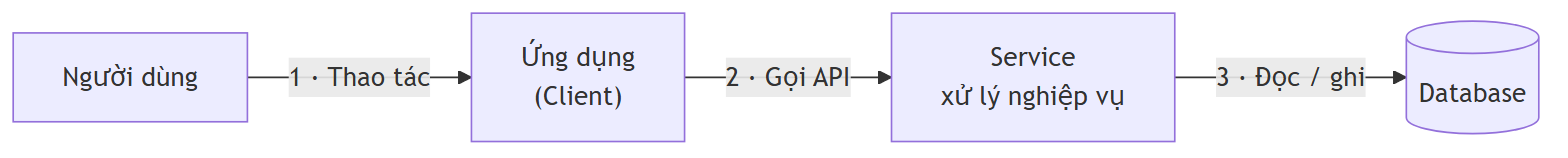
\includegraphics[width=0.85\textwidth]{vi-du-kien-truc.png}
  \caption{Ví dụ sơ đồ sinh từ \texttt{mermaid\_src/vi-du-kien-truc.mmd}}
  \label{fig:vi-du-kien-truc}
\end{figure}

\section{Ví dụ bảng}
\label{sec:vi-du-bang}

\begin{table}[H]
  \centering
  \begin{tabularx}{\textwidth}{@{}l X@{}}
    \toprule
    \textbf{Thuộc tính} & \textbf{Ý nghĩa} \\
    \midrule
    \texttt{user\_id} & Cột trái ngắn (\texttt{l}), cột phải tự xuống dòng (\texttt{X}). \\
    \texttt{is\_active} & Tham chiếu chéo: Hình~\ref{fig:vi-du-kien-truc}. \\
    \bottomrule
  \end{tabularx}
  \caption{Ví dụ bảng hai cột}
  \label{tab:vi-du}
\end{table}
% ---- HẾT NỘI DUNG MẪU ----


% ==== Phụ lục -- tạo sections/99-phu-luc.tex rồi bỏ comment ====
% \appendix
% \input{sections/99-phu-luc}

\end{document}
